\documentclass[11pt]{article}
\usepackage[utf8]{inputenc}
\usepackage{amsmath,amssymb,hyperref,array,xcolor,multicol,verbatim,mathpazo}
\usepackage[normalem]{ulem}
\usepackage[pdftex]{graphicx}
\usepackage{fullpage}


\usepackage[backend=biber,style=authoryear,
sorting=ynt,citestyle=authoryear]{biblatex}
\addbibresource{papercitations.bib}
\usepackage{setspace}
\onehalfspacing
\addtolength{\skip\footins}{2pc plus 5pt}

\title{Progress on Event Study Graphs}
%\author{Hanna Glenn}
%\date{\today}

\DeclareLabeldate[online]{%
  \field{date}
  \field{year}
  \field{eventdate}
  \field{origdate}
  \field{urldate}
}





\begin{document}

\textbf{Progress on Event Study Graphs}

\vspace{2cm}

\centering

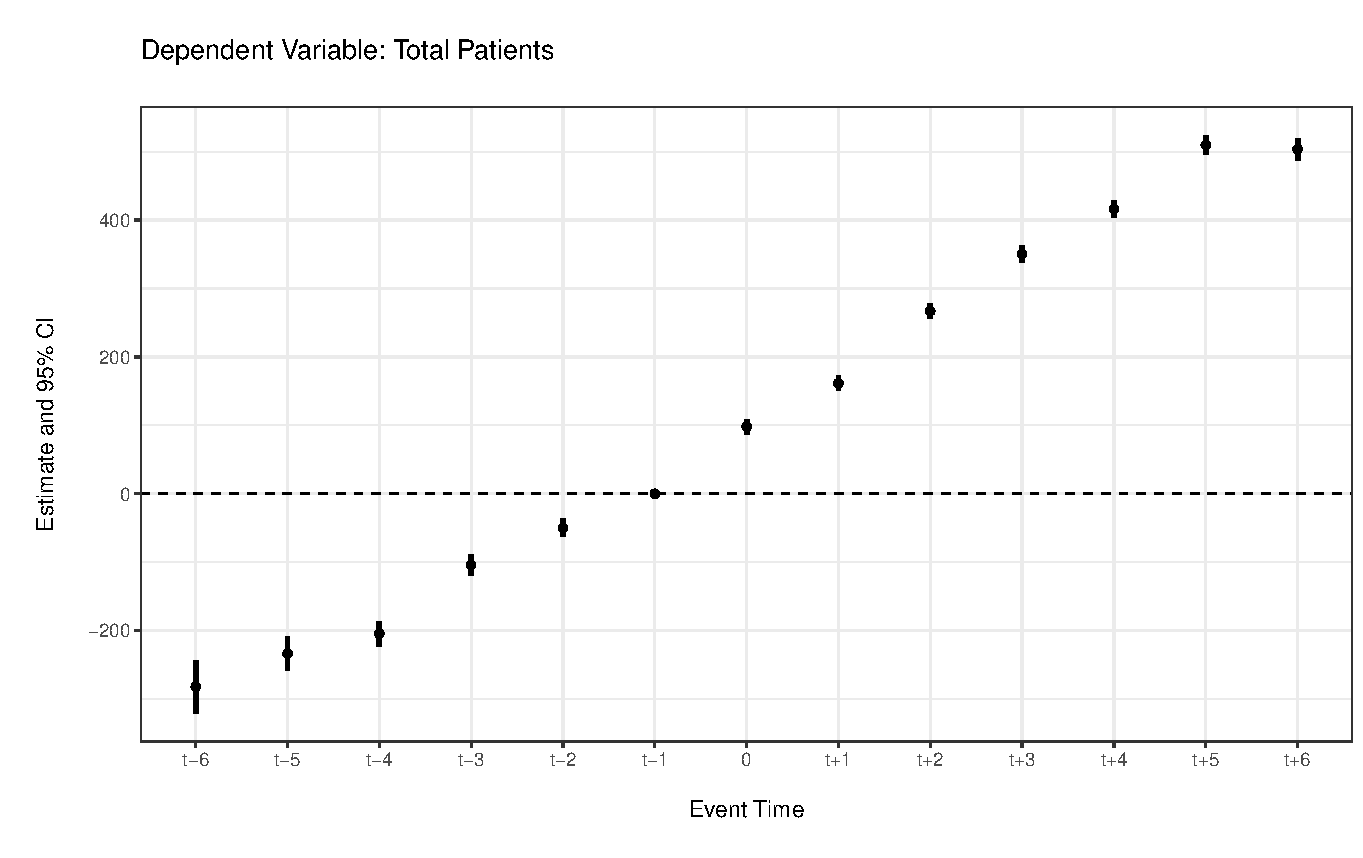
\includegraphics[scale=.7]{Objects/cont_ES_fullsample.pdf}
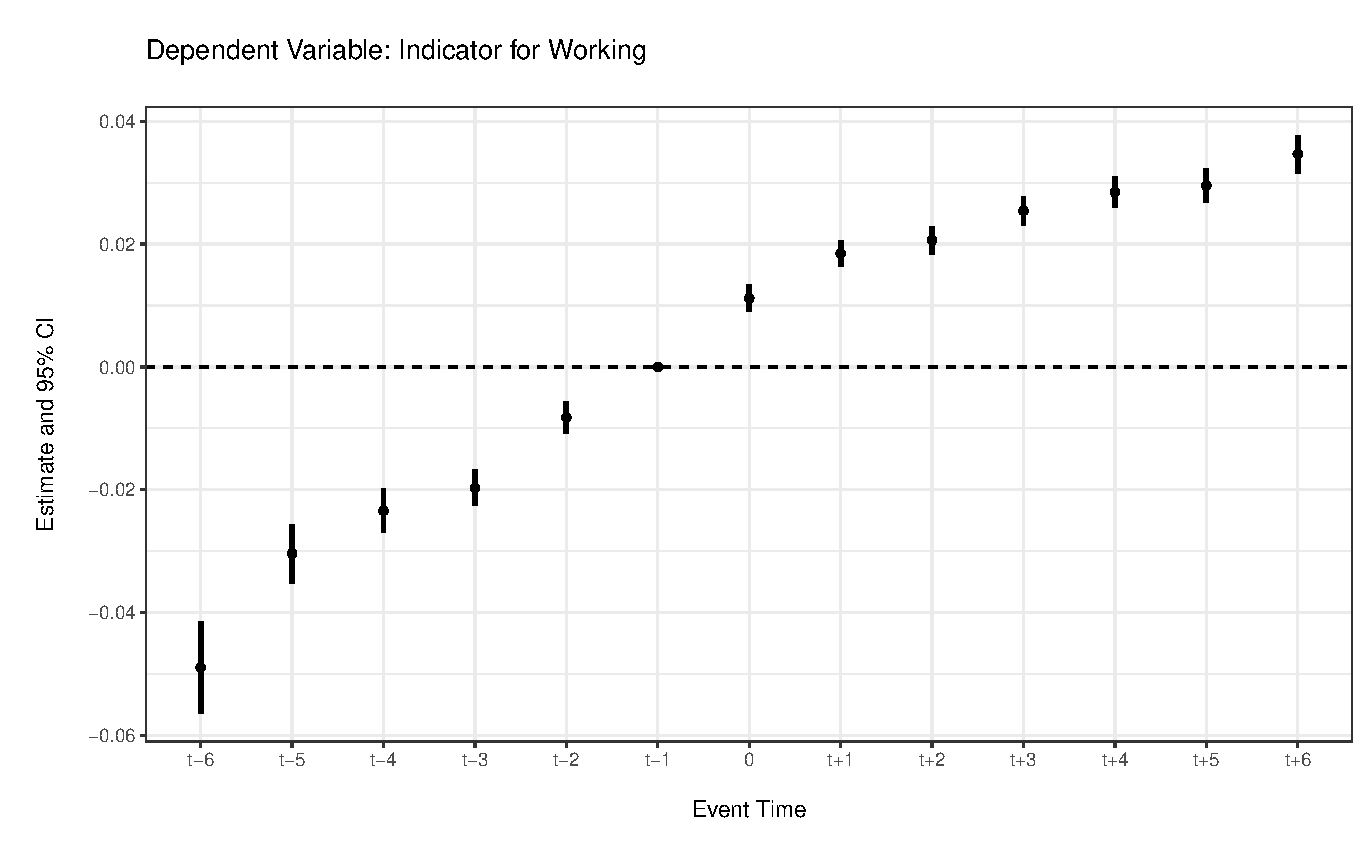
\includegraphics[scale=.7]{Objects/ind_ES_fullsample.pdf}
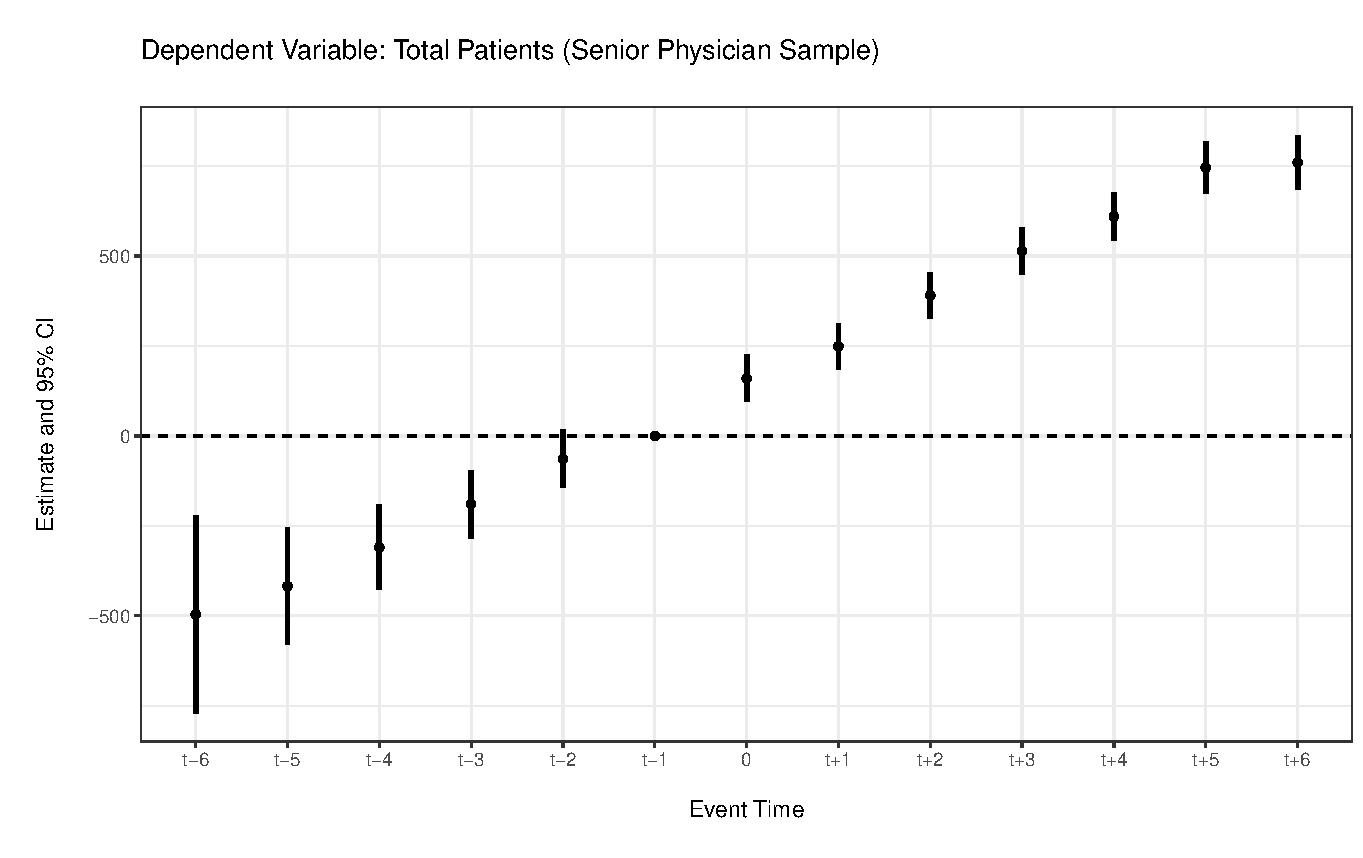
\includegraphics[scale=.7]{Objects/cont_ES_oldsample.pdf}
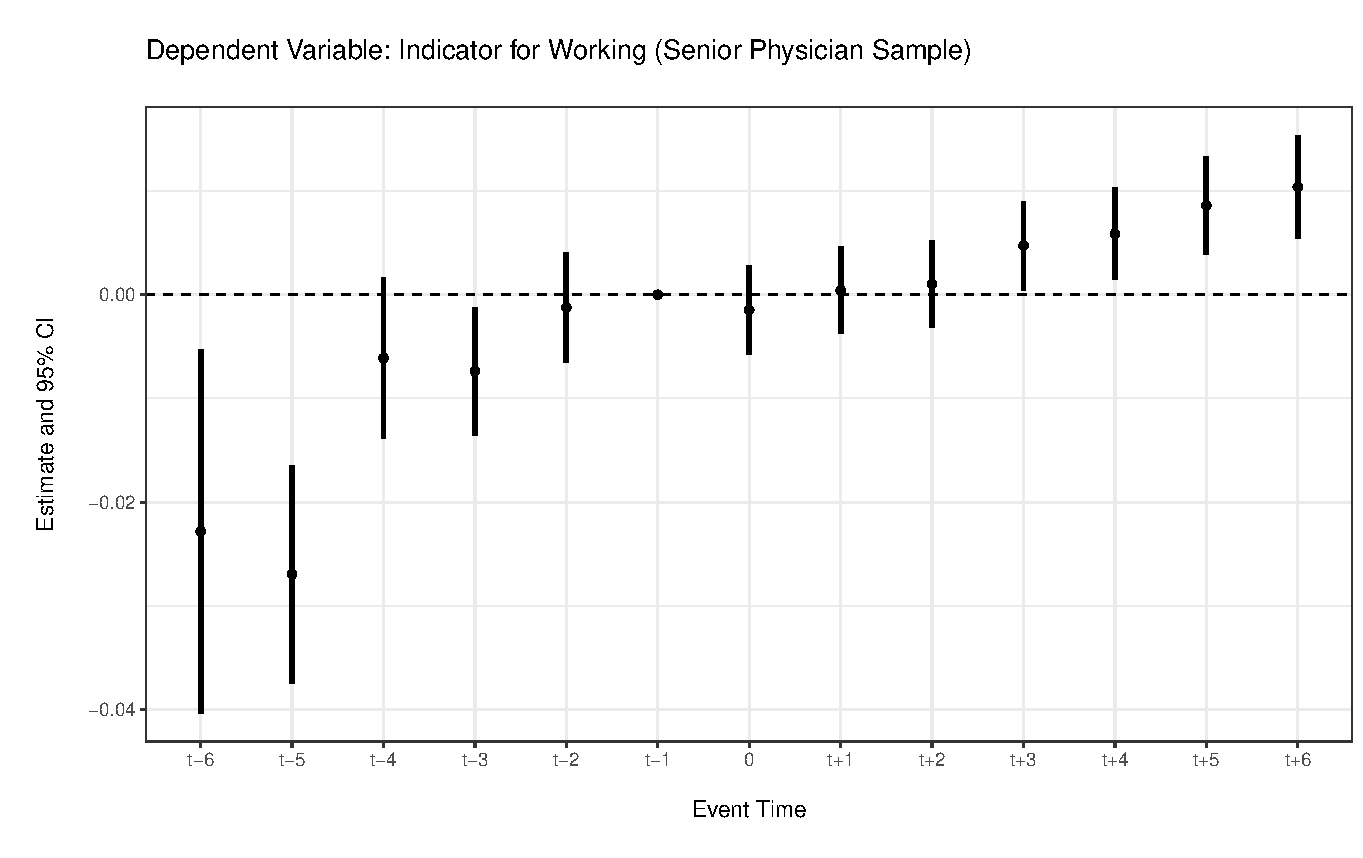
\includegraphics[scale=.7]{Objects/ind_ES_oldsample.pdf}

\newpage

A large proportion of physicians were exposed to EHR hospitals in 2009. I wasn't entirely sure how to think about these observations in the analysis so I also included two graphs where those observations are dropped completely. 

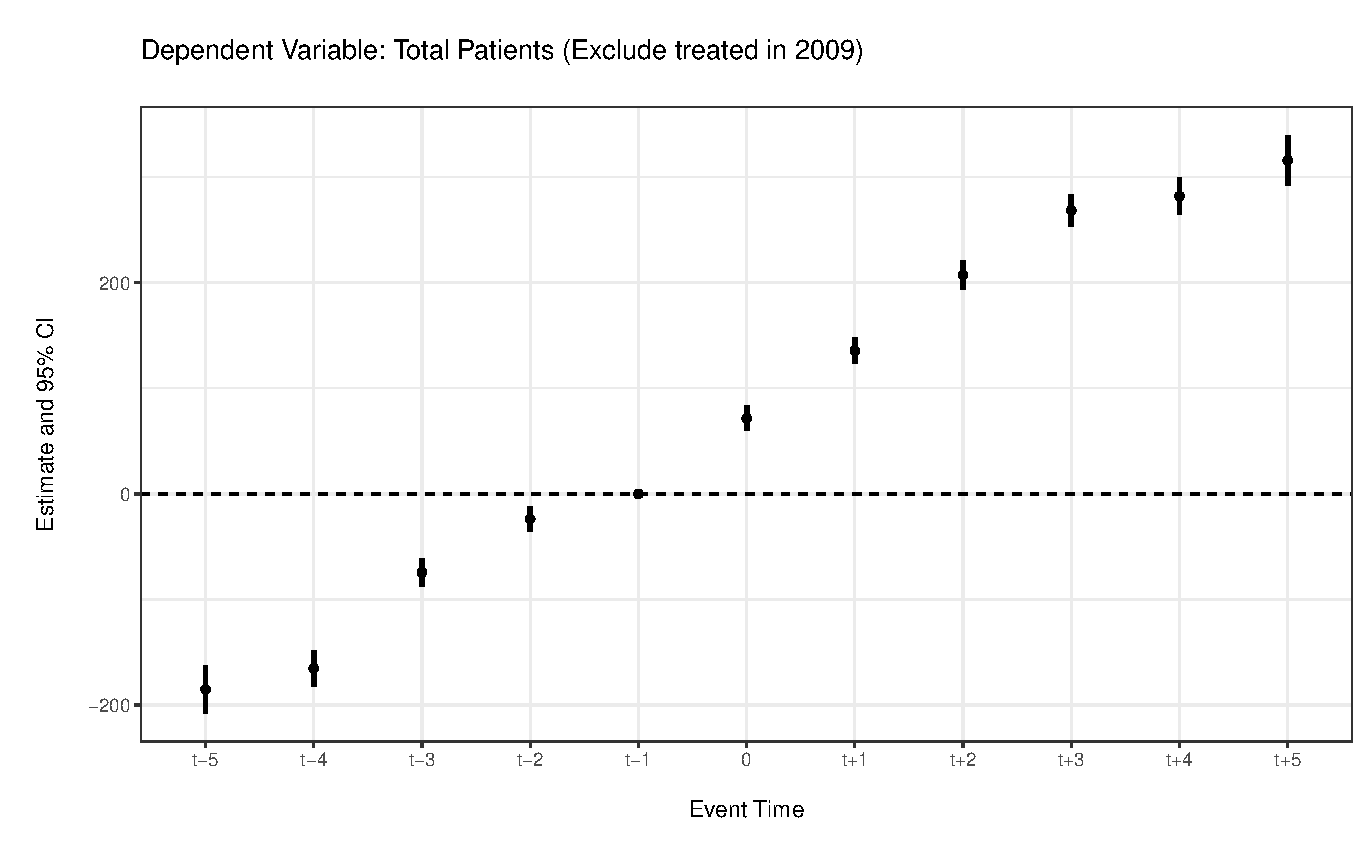
\includegraphics[scale=.7]{Objects/cont_ES_subset2009.pdf}
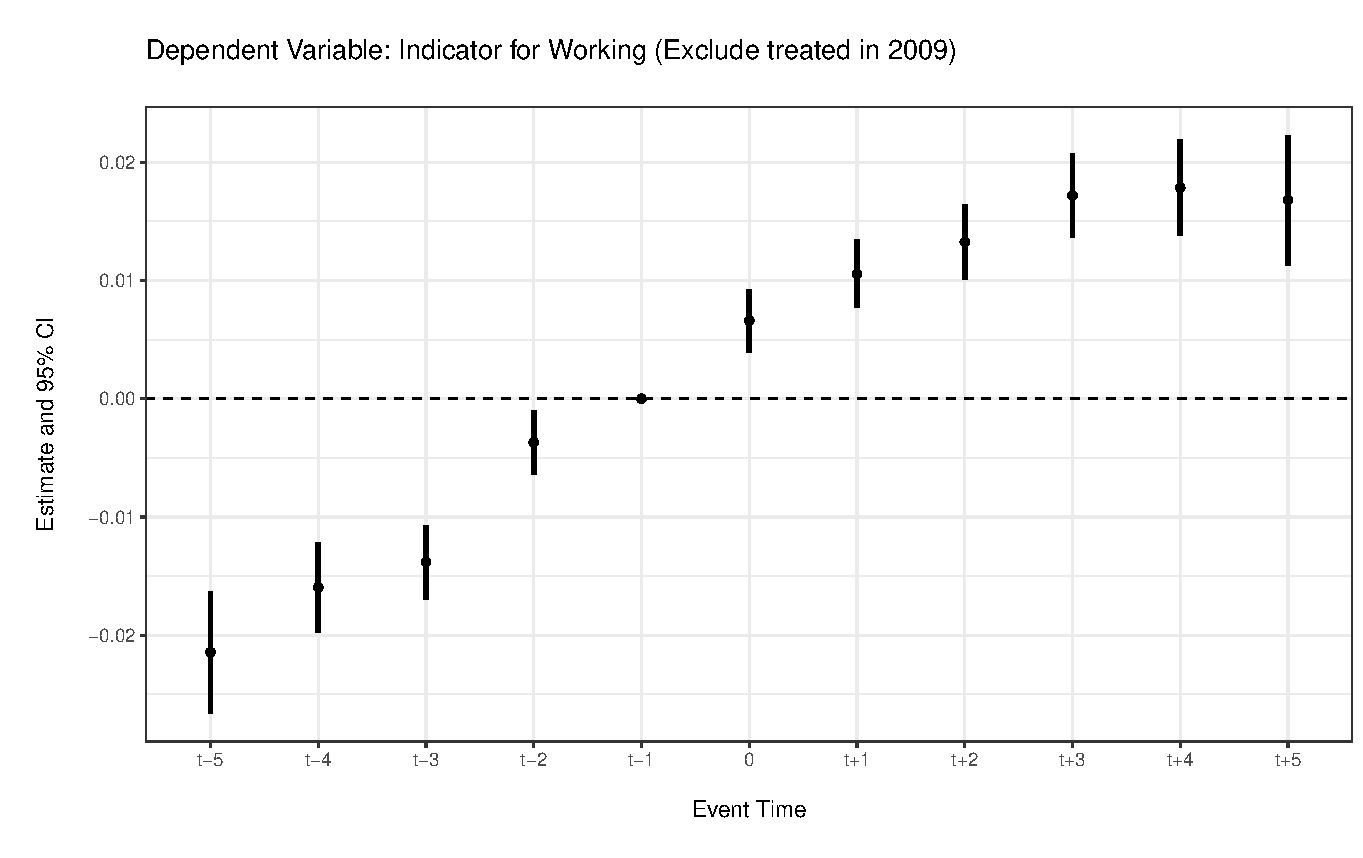
\includegraphics[scale=.7]{Objects/ind_ES_subset2009.pdf}




\end{document}